\chapter{Chordal graphs}

\section{Introduction}

A graph $G$ is chordal, if it does not contain an induced cycle of length $\geq 4$. Equivalently, if every cycle $C$ of length $\geq 4$ in $G$ contains a chord.

A \emph{perfect elemination ordering} is an ordering $v_1, v_2, \dots, v_n$ of vertices of $G$ so that $v_i$ is \emph{simplicial vertex} in $G[v_{i}, v_{i+1}, \dots, v_n]$, i.e., $v_i$ and neighbors after it in the ordering form a clique.

A graph $G$ is chordal if and only if it admits a perfect elimination ordering.

\section{Implementation}

\begin{enumerate}
\item Implement \verb`max_cardinality_search(G)` which returns PEO of $G$ using maximal cardinality search algorithm (see \href{http://matematika.fri.uni-lj.si/dm/discrete_mathematics.pdf}{Lecture notes}, Algorithm 7.1.).
\item Write function \verb`is_chordal(G)` which checks if graph $G$ is chordal. Use algorithm 7.2 from Lecture notes. See also comments in the code below.
\item Write function \verb`color_chordal_graph(G)` which returns minimal (optimal) coloring of chordal graph $G$. See Lecture notes.
\end{enumerate}

\begin{sageCell}
def max_cardinality_search(G):
    """
    Maximum cardinality search
    """
    mcs = []
    white = set(G.vertices(sort=False))
    black = set()
    while len(white) > 0:
        maxw = max(white, key = lambda w: len([v for v in G.neighbors(w) if v in black]))
        mcs = [maxw] + mcs
        black.add(maxw)
        white.remove(maxw)
    return mcs

def is_chordal(G):
    """
    Test if graph G is chordal.

    """
    peo = max_cardinality_search(G)
    # We need to check that max_cardinality_search really returns perfect elimination ordering (PEO)
    # let peo be = [v0, v1, ... v{n-1}]
    # for i = 0 ... n-1:
    #    for vi find j > i such that vj is neighbor of vi and j is as small as possible
    #    then, for all vk which are neighbors of vi, k > j, vj and vk must be adjacent
    indexmap = dict(zip(peo, range(len(peo))))
    # v is vi in Algorithm 7.2
    for v in peo:
        # sorted list of peo indexes of "right" neighbors of v
        vnindexes = sorted([indexmap[w] for w in G.neighbors(v) if indexmap[w] > indexmap[v]])
        if len(vnindexes) > 0:
            # u is the first "right" neighbor of v in peo (vj in Algorithm 7.2)
            u = peo[vnindexes[0]]
            for wi in vnindexes[1:]:
                if not G.has_edge(u, peo[wi]):
                    return False
    return True

def color_chordal_graph(G):
    """
    Optimally color chordal graph G.
    """
    col = {}
    peo = max_cardinality_search(G);
    # Algorithm is greedy and efficient:
    #   go from the last to the first vertex in peo
    #   select the first available color for v (smallest not used by right neighbors)
    # Thus, for chordal graphs optimal coloring is "easy" problem!
    indexmap = dict(zip(peo, range(len(peo))))
    colors = range(len(peo))
    # go from the last to the first vertex in peo
    for v in reversed(peo):
        # colors of right neighbors
        vncol = set([col[w] for w in G.neighbors(v) if indexmap[w] > indexmap[v]])
        # select the first available color for v (smallest not used by right neighbors)
        col[v] = next(enumerate(c for c in colors if c not in vncol))[1]
    return col
\end{sageCell}

\subsection*{Examples}

\begin{sageCell}
def random_chordal_graph(n, kmin = 5, kmax = 10, kidmin = 2, kidmax = 4):
    """Returns a 'random' chordal graph.
    The sizes of maximal cliques are between `kmin` and `kmax`,
    the intersections of maximal cliques are between `kidmin` and `kidmax`."""
    from random import randint, sample

    G = Graph()
    cliques = []
    nG = 0

    # create cliques
    for i in range(n):
        s = randint(kmin, kmax)
        K = graphs.CompleteGraph(s)
        K.relabel(lambda w: w + nG)
        G = G.union(K)
        cliques.append(K.vertices(sort=False))
        nG += s

    # merge parts of cliques
    for i in range(1, n):
        j = randint(0, i - 1)
        C1 = cliques[j]
        C2 = cliques[i]
        nmin = min(len(C1), len(C2))
        k = randint(kidmin, min(kidmax, nmin - 1))
        iC1 = sample(C1, k)
        iC2 = sample(C2, k)
        id = zip(iC1, iC2)
        for (u, v) in id:
            G.merge_vertices((u, v))
            C2 = [u if x == v else x for x in C2]
        cliques[i] = C2
    return G
\end{sageCell}

\begin{sageCell}
    def apollonian_network(n):
    """Apollonian network is a graph formed by a process of recursively subdividing a triangle
    into three smaller triangles. This function returns Apollonian network on n vertices, n >= 3."""
    from random import choice
    G = graphs.CycleGraph(3)
    pos = {0: [1, 0], 1: [-0.5, 0.866], 2: [-0.5, -0.866]}
    faces = [[0, 1, 2]]
    for i in range(3, n):
        f = choice(faces)
        x, y, z = f
        faces.remove(f)
        faces.extend([[x, y, i], [i, y, z], [i, z, x]])
        G.add_edges([(x, i), (y, i), (z, i)])
        xi = sum(a for (a, b) in [pos[w] for w in [x, y, z]])/3
        yi = sum(b for (a, b) in [pos[w] for w in [x, y, z]])/3
        pos[i] = (xi, yi)
    G.set_pos(pos)
    return G
\end{sageCell}

\begin{sageCell}
    G = random_chordal_graph(3)
    max_cardinality_search(G), is_chordal(G)
\end{sageCell}
\begin{outCell}
    ([22, 19, 17, 16, 15, 14, 13, 8, 7, 6, 5, 4, 3, 2, 1, 0], True)
\end{outCell}

\begin{sageCell}
    is_chordal(graphs.CompleteGraph(4))
\end{sageCell}
\begin{outCell}
    True
\end{outCell}

\begin{sageCell}
    is_chordal(graphs.CycleGraph(4))
\end{sageCell}
\begin{outCell}
    False
\end{outCell}

\begin{sageCell}
def color_graph(G, coloring, **kwargs):
    all_colors = list(colors)[10:];
    color_map = {}
    for v, c in coloring.items():
        color = all_colors[c]
        color_map.setdefault(color, []).append(v)
    return G.plot(vertex_colors=color_map, **kwargs)
\end{sageCell}
\begin{sageCell}
    G = apollonian_network(10)
    coloring = color_chordal_graph(G)
    color_graph(G, coloring)
\end{sageCell}

\begin{outImage}
   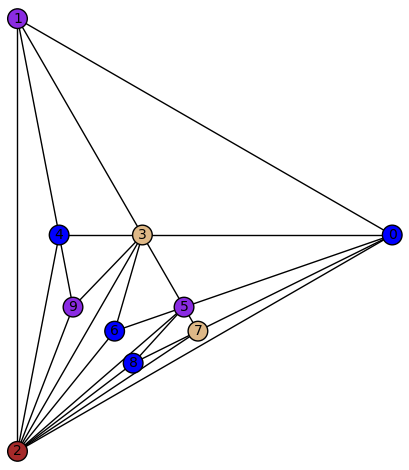
\includegraphics[width=0.6\textwidth]{Images/ChordalGraphs/apollonian_network.png}
\end{outImage}

